\section{Was sind Differentialgleichungen?}

\subsection{Einführungsbeispiel}

\begin{minipage}[t]{0.76\textwidth}
    \vspace{0pt}
    Denken Sie sich ein quaderförmiges Gefäss mit einem
    Quadrat der Seitenlänge \SI{1}{\deci\meter} als
    Grundfläche und einer Höhe von \SI{4}{\deci\meter}
    (Bild rechts). Zu Beginn ist das Gefäss ganz mit
    Wasser gefüllt. Im Boden gibt es eine kleine Öffnung
    mit einem Querschnitt von
    \[
        \SI{0.005}{\square\deci\meter}
        = \frac{1}{200}\,\mathrm{dm}^2.
    \]
\end{minipage}
\hfill
\begin{minipage}[t]{0.21\textwidth}
    \vspace{0pt}
    \centering
    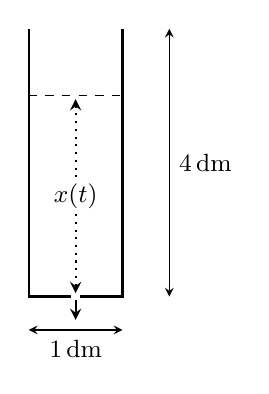
\begin{tikzpicture}[
            >=stealth,
            scale=0.85,
            every node/.style={font=\small}
        ]
        % Gefäss
        \draw[thick] (0,4) -- (0,0) -- (1.4,0) -- (1.4,4);

        % Wasserstand
        \draw[dashed] (0,3) -- (1.4,3);

        % Wasserhöhe x(t)
        \draw[<->,dotted,thick]
        (0.7,0.05) -- (0.7,2.95);
        \node[fill=white,inner sep=2pt]
        at (0.7,1.5) {\(x(t)\)};

        % Gesamthöhe
        \draw[<->] (2.1,0) -- (2.1,4);
        \node[right] at (2.1,2) {\(4\,\mathrm{dm}\)};

        % Breite
        \draw[<->] (0,-0.5) -- (1.4,-0.5);
        \node[below] at (0.7,-0.5) {\(1\,\mathrm{dm}\)};

        % Ausflussöffnung
        \fill[white] (0.63,-0.04)
        rectangle (0.77,0.04);
        \draw[->,thick] (0.7,-0.05) -- (0.7,-0.35);
    \end{tikzpicture}
\end{minipage}

Durch die Öffnung fliesst Wasser aus dem Gefäss.
Die Geschwindigkeit, mit der das Wasser ausfliesst,
verändert sich jedoch mit der Zeit: Je niedriger
der Wasserstand, desto kleiner die Austrittsgeschwindigkeit.
Evangelista Torricelli (1608--1647) hat dieses Problem
untersucht und den folgenden Zusammenhang zwischen
Wasserstand und Austrittsgeschwindigkeit
(in \si{\deci\meter\per\second}) gefunden:
\[
    v = \sqrt{2gx}
\]
Dabei ist \(g=\SI{98.1}{\deci\meter\per\second\squared}\)
die Erdbeschleunigung und \(x\) die Wasserhöhe in
Dezimetern. Mit der Näherung
\(g\approx\SI{100}{\deci\meter\per\second\squared}\)
folgt:
\[
    v = \sqrt{200\cdot x}
\]
Wie kann man damit berechnen, wie lange es dauert,
bis sich das Gefäss vollständig geleert hat?

Da sich der Wasserstand im Laufe der Zeit verändert,
handelt es sich bei \(x\) um eine Funktion der Zeit:
\(x=x(t)\). Da zu Beginn das Gefäss voll ist, gilt
\(x(0)=4\). Das nennt man eine \textbf{Anfangsbedingung}.

Ausserdem lässt sich mit der Formel zur
Austrittsgeschwindigkeit eine Aussage zur Ableitung
\(\dot{x}(t)\) der Funktion \(x(t)\) machen:

\clearpage

\textit{Herleitung der Differentialgleichung in der Klasse \dots}

\karofeld{20}

\clearpage


\begin{ueb}{Aufgaben zum Einführungsbeispiel}{ueb:einfuehrung}

    \begin{enumerate}
        \item \textbf{Zur Lösung des Problems}

              \begin{enumerate}
                  \item Zeigen Sie, dass die Funktion
                        \[
                            x(t)=\left(c-\frac{1}{\sqrt{800}}\,t\right)^2
                        \]
                        die Differentialgleichung
                        \[
                            \dot{x}(t)=-\sqrt{\frac{x(t)}{200}}
                        \]
                        löst, indem Sie \(x\) in beide Seiten der Gleichung
                        einsetzen, diese separat vereinfachen und die Ergebnisse
                        am Schluss vergleichen. Dabei ist \(c\) eine beliebig
                        wählbare (positive) Zahl.

                  \item Bestimmen Sie \(c>0\) so, dass \(x(t)\) die
                        Anfangsbedingung \(x(0)=4\) erfüllt.

                  \item Zeichnen Sie den Graphen von \(x(t)\)
                        (z.\,B. mit GeoGebra) und berechnen Sie die
                        Entleerungszeit.
              \end{enumerate}

        \item \textbf{Das Problem wird angepasst}

              \begin{enumerate}
                  \item Wie ändert sich die Differentialgleichung,
                        wenn das Problem wie folgt abgeändert wird?

                        Aus einem Wasserhahn fliesst Wasser ins Gefäss,
                        und zwar mit einer konstanten Rate von
                        \SI{0.12}{\liter\per\second}.

                  \item Untersuchen Sie, ob die in a) gefundene
                        Differentialgleichung eine konstante Lösung
                        besitzt, also eine Lösung der Form
                        \[
                            x(t)=x^*.
                        \]
                        Dabei ist \(x^*\) eine Konstante, die Sie finden
                        können, indem Sie \(x(t)=x^*\) in die
                        Differentialgleichung einsetzen.

                        Eine solche Lösung heisst
                        \textbf{Gleichgewichtslösung}.

                        Wie muss man diese Lösung physikalisch
                        interpretieren?

                  \item Die Lösung der Differentialgleichung aus a)
                        mit der Anfangsbedingung \(x(0)=1\) ist
                        unten dargestellt.

                        Interpretieren Sie Ihr in Aufgabe b)
                        gefundenes Resultat im Lichte der Abbildung.


                        \begin{center}
                            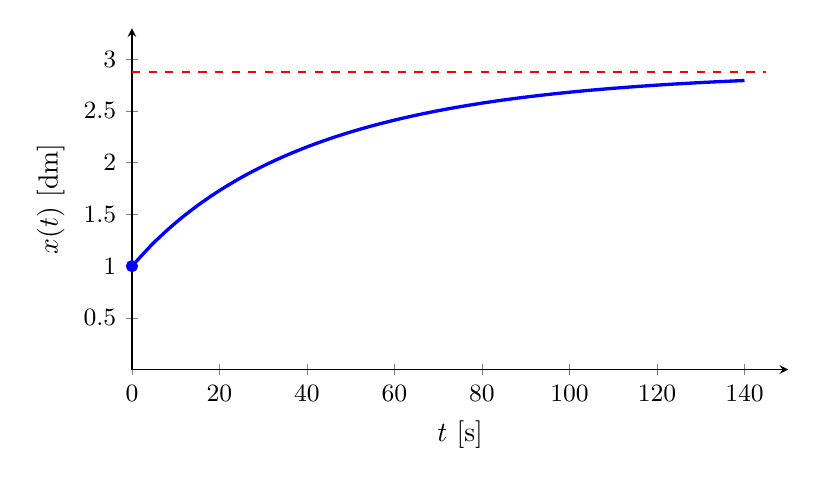
\begin{tikzpicture}
                                \begin{axis}[
                                        width=12cm,
                                        height=7cm,
                                        axis lines=left,
                                        xmin=0, xmax=150,
                                        ymin=0, ymax=3.3,
                                        xtick={0,20,...,140},
                                        ytick={0.5,1,1.5,2,2.5,3},
                                        xlabel={\(t\) [s]},
                                        ylabel={\(x(t)\) [dm]},
                                        %xlabel style={at={(axis description cs:1,0)},anchor=north east},
                                        %ylabel style={at={(axis description cs:0,1)},anchor=south east},
                                        tick label style={font=\small},
                                        clip=false,
                                        scale = 0.8
                                    ]

                                    % Numerische Lösung (Runge-Kutta 4. Ordnung)
                                    \addplot[
                                        blue,
                                        very thick,
                                        smooth
                                    ] coordinates {
                                            (0,1.000000)
                                            (5,1.226588)
                                            (10,1.419619)
                                            (15,1.585970)
                                            (20,1.730500)
                                            (25,1.856835)
                                            (30,1.967785)
                                            (35,2.065590)
                                            (40,2.152068)
                                            (45,2.228725)
                                            (50,2.296819)
                                            (55,2.357413)
                                            (60,2.411416)
                                            (65,2.459607)
                                            (70,2.502660)
                                            (75,2.541160)
                                            (80,2.575619)
                                            (85,2.606483)
                                            (90,2.634145)
                                            (95,2.658953)
                                            (100,2.681212)
                                            (105,2.701193)
                                            (110,2.719136)
                                            (115,2.735255)
                                            (120,2.749739)
                                            (125,2.762760)
                                            (130,2.774466)
                                            (135,2.784993)
                                            (140,2.794463)
                                        };

                                    % Gleichgewichtslösung
                                    \addplot[
                                        red,
                                        dashed,
                                        thick,
                                        domain=0:145
                                    ] {2.88};

                                    % \node[
                                    %     red,
                                    %     anchor=south east
                                    % ] at (axis cs:145,2.88)
                                    % {\(x^*=2.88\)};

                                    % Anfangsbedingung
                                    \addplot[
                                        blue,
                                        only marks,
                                        mark=*,
                                        mark size=2pt
                                    ] coordinates {(0,1)};

                                \end{axis}
                            \end{tikzpicture}
                        \end{center}

              \end{enumerate}
    \end{enumerate}

\end{ueb}


\clearpage

\subsection*{Lösungen}

\begin{enumerate}
    \item \textbf{Lösung des Problems}

          \begin{enumerate}
              \item Durch Einsetzen von \(x(t)\) erhält man auf beiden
                    Seiten der Gleichung den gleichen Term.

                    Nützlich dabei ist die Umformung
                    \(\sqrt{800}=2\cdot\sqrt{200}\).

              \item \(c=2\)

              \item Entleerungszeit:
                    \(2\cdot\sqrt{800}\) Sekunden
                    \(\approx \SI{56.6}{\second}\).
          \end{enumerate}

    \item \textbf{Neues Problem mit Zulauf}

          \begin{enumerate}
              \item Analog zur Herleitung der ursprünglichen
                    Differentialgleichung folgt
                    \[
                        \dot{x}(t)
                        =-\sqrt{\frac{x(t)}{200}}+0.12.
                    \]

              \item \(x^*=2.88\)

                    % Bei dieser Wasserhöhe sind Zu- und Abfluss
                    % gleich gross. Der Wasserstand bleibt deshalb
                    % konstant.

              \item \dots
                    %Die Lösung nähert sich mit zunehmender Zeit
                    %         der Gleichgewichtslösung \(x^*=2.88\) an.

                    %         Da der anfängliche Wasserstand \(x(0)=1\)
                    %         unterhalb des Gleichgewichtswerts liegt,
                    %         steigt der Wasserstand zunächst an.
                    %         Die Zunahme wird mit der Zeit immer kleiner.
                    %         Der Graph nähert sich asymptotisch der
                    %         horizontalen Geraden \(x=2.88\).
          \end{enumerate}
\end{enumerate}











\clearpage
\subsection{Grundbegriffe}

\begin{definition}{Differentialgleichung und Ordnung}{def:dgl}
    Eine \textbf{Differentialgleichung} ist eine Gleichung, in der
    eine unbekannte Funktion und ihre Ableitungen vorkommen.

    Die \textbf{Ordnung} einer Differentialgleichung ist die
    Ordnung der höchsten auftretenden Ableitung der gesuchten Funktion.
\end{definition}

Wir werden im Hinblick auf die Anwendungen die unabhängige Variable
häufig mit \(t\) bezeichnen und die gesuchte Funktion mit \(x(t)\).
Differentialgleichungen haben dann beispielsweise die Form
\[
    \begin{aligned}
        \dot{x}(t)             & = -3x(t)
                               & \qquad
        \ddot{x}(t)+x(t)       & = 0             \\[6pt]
        x^{(4)}(t)             & = 3t+1
                               & \qquad
        \ddot{x}(t)+\dot{x}(t) & = x(t)+3\cos(t)
    \end{aligned}
\]
Weit verbreitet ist auch die Schreibweise
\(y'(x)=-3y(x)\), wobei dann \(x\) die unabhängige Variable
ist und die Funktion \(y(x)\) gesucht wird.

Differentialgleichungen haben häufig \emph{unendlich viele Lösungen}.
Das kann man leicht an einem Beispiel erkennen.
Betrachten wir dazu die Differentialgleichung
\[
    \dot{x}(t)=\cos(t).
\]
Gesucht ist eine Funktion \(x(t)\) mit der Ableitung
\(\cos(t)\). Davon gibt es viele!
Ein Beispiel wäre \(x(t)=\sin(t)\).
Ein anderes \(x(t)=\sin(t)+42\).
Allgemein sind alle Funktionen der Form
\[
    x(t)=\sin(t)+c, \qquad c\in\R,
\]
Lösungen dieser Differentialgleichung.

Wenn wir aber nach einer Lösung suchen, die zusätzlich
die Eigenschaft hat, dass \(x(0)=27\) ist, dann gibt es
nur noch eine gültige Lösung:
\(x(t)=\sin(t)+27\).

Eine solche Zusatzbedingung nennt man eine
\textbf{Anfangsbedingung} (der Wert zur Zeit \(t=0\)).
Eine Differentialgleichung mit vorgegebener Anfangsbedingung
nennt man dann ein \textbf{Anfangswertproblem}.

Differentialgleichungen, die nach der höchsten Ableitung
der Funktion aufgelöst sind, nennt man
\emph{explizite}, die anderen \emph{implizite}
Differentialgleichungen.


Betrachten Sie die vier Differentialgleichungen von oben.
Sind es implizite oder explizite
Differentialgleichungen?
Was ist jeweils ihre Ordnung?
Können Sie jeweils eine Lösung angeben?


\begin{ueb}{Lösungen von Differentialgleichungen überprüfen}{ueb:loesungen_ueberpruefen}
    Zeigen Sie durch Einsetzen, dass die Funktion \(x(t)\) für jede
    Wahl des Parameters \(c\) eine Lösung der angegebenen
    Differentialgleichung ist.

    Bestimmen Sie anschliessend den Wert von \(c\), sodass die
    Lösung auch die angegebene Anfangsbedingung erfüllt.

    \begin{enumerate}
        \item
              \[
                  \dot{x}(t)=1+t-x(t), \qquad
                  x(t)=t+ce^{-t}, \qquad
                  x(0)=7
              \]

        \item
              \[
                  \dot{x}(t)=\frac{3x(t)}{t}+t, \qquad
                  x(t)=ct^3-t^2, \qquad
                  x(1)=3
              \]

        \item
              \[
                  t\cdot\dot{x}(t)+x(t)=\sin(t), \qquad
                  x(t)=\frac{1}{t}(c-\cos(t)), \qquad
                  x(\pi)=0
              \]
    \end{enumerate}
\end{ueb}


\textit{Kurzlösungen:} a) \(c=7\), b) \(c=4\), c) \(c=-1\).
